\subsection{\texorpdfstring{\nitrogen{}}{15N} HMQC}
\label{subsec:noah__hmqc}

In \cref{subsec:noah__sehsqc_n}, I will discuss how the sensitivity-enhanced HSQC modules developed above may be adapted into \proton{}--\nitrogen{} experiments.
However, before that, I make a slight detour to cover the \nitrogen{} HMQC experiment, which (up until my DPhil) was the experiment of choice for detecting one-bond \proton{}--\nitrogen{} correlations.

\begin{figure}[htb]
    \centering
    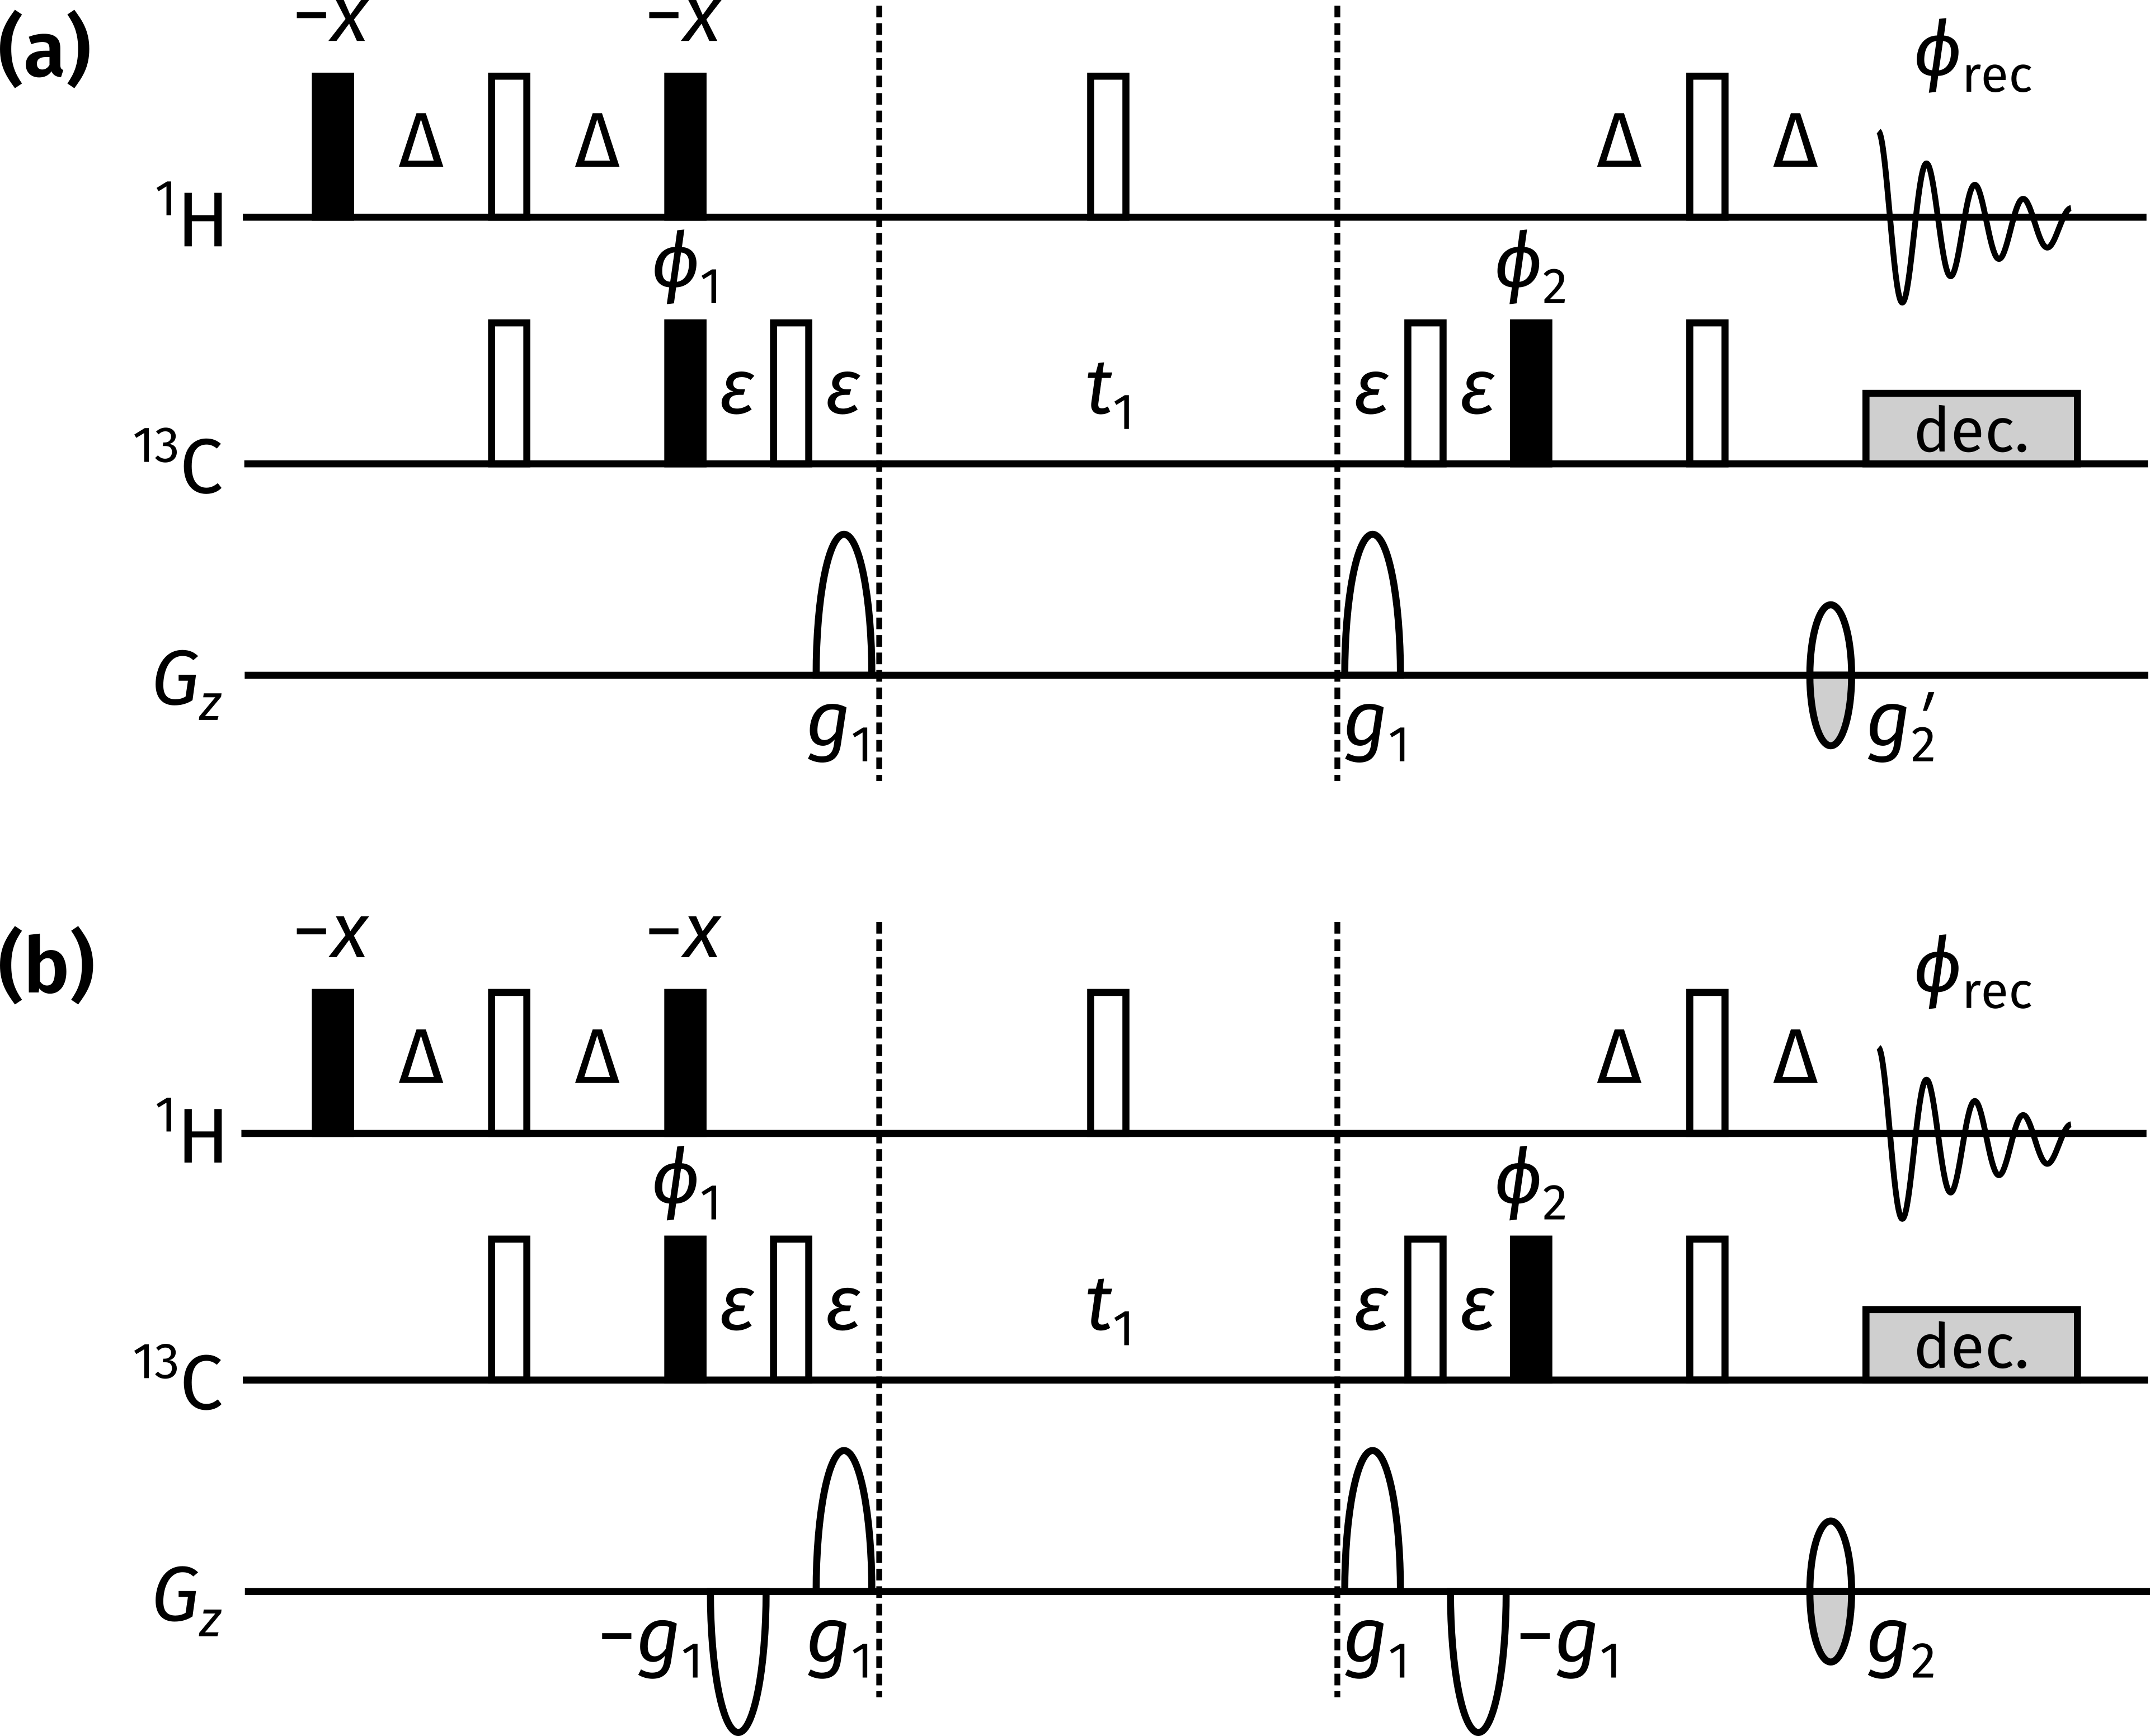
\includegraphics[]{pp/hmqc/all.png}%
    {\phantomsubcaption\label{fig:noah_hmqc_2grad}}%
    {\phantomsubcaption\label{fig:noah_hmqc_4grad}}%
    \caption[NOAH HMQC pulse sequences]{
        \textbf{(\subref*{fig:noah_hmqc_2grad})} With two encoding gradients around $t_1$.
        \textbf{(\subref*{fig:noah_hmqc_4grad})} With four encoding gradients around $t_1$.
        Phase cycling is performed with $\phi_1 = (x, -x)$, $\phi_2 = (x, x, -x, -x)$, and $\phi_\text{rec} = (x, -x, -x, x)$.
        The delay $\Delta$ is set to $1 / (4 \cdot \oneJ{NH})$.
        Gradient amplitudes are: $g_1 = 80\%$; $g_2 = \pm 32.4\%$; $g_2' = g_2/2$.
    }
    \label{fig:noah_hmqc}
\end{figure}


\subsubsection{CTP gradient scheme}

The HMQC module is based on the ASAP-HMQC reported by Kup{\v{c}}e and Freeman\autocite{Kupce2007MRC}, which used a symmetric gradient scheme similar to that in the seHSQC modules previously described (\cref{fig:noah_hmqc_2grad}).
However, in the NOAH module\autocite{Kupce2017ACIE}, bipolar gradient pulse pairs were placed before and after $t_1$ (\cref{fig:noah_hmqc_4grad}).
This was likely implemented in order to allow the final gradient, $g_2$, to have as large an amplitude as possible.
In heteronuclear experiments, this final gradient is particularly important for dephasing bulk magnetisation which is transverse just prior to detection (due to pulse imperfections or relaxation).
If this gradient is too weak, this unwanted magnetisation will be incompletely dephased, leading to artefacts in the resulting spectrum.

Strategies to maximise this gradient amplitude are particularly crucial in \proton{}--\nitrogen{} experiments (as compared to \proton{}--\carbon{} experiments) for two reasons.
Firstly, the natural abundance of \nitrogen{} (0.36\%) is even smaller than \carbon{} (1.1\%), meaning that better suppression must be achieved in order for the artefacts to not obscure the signal.
Secondly, the gyromagnetic ratio of \nitrogen{} is also smaller: thus, since $g_2/g_1 \propto \gammaN/\gammaH$, an unmodified pulse sequence will naturally have a smaller $g_2$.

In this respect, the four-gradient scheme in \cref{fig:noah_hmqc_4grad} is superior to the two-gradient scheme, because the gradient $g_2$ will have an amplitude of $4\gammaN g_1/\gammaH$.
However, when used in a NOAH supersequence, this leads to wing artefacts in downstream modules, since bulk \magnnot{N} magnetisation effectively does not experience any coherence order selection during $t_1$.
This motivates a return to the two-gradient scheme of \cref{fig:noah_hmqc_2grad}.
To compensate for the fact that the decoding gradient $g_2'$ has half of the amplitude of $g_2$, all CTP gradients were instead \textit{lengthened} from their usual duration of \qty{1}{\ms} to \qty{2.5}{\ms}.
This ensures that any stray transverse bulk magnetisation at the end of the HMQC module is effectively dephased.

The HMQC spectra thus obtained are shown in \cref{fig:hmqc_grad_spec}.
These, and all other \proton{}--\nitrogen{} spectra in this chapter, were acquired assuming a $\oneJ{NH}$ value of \qty{90}{\Hz}.
The first column shows the spectra obtained with the original four-gradient scheme: although the artefacts at \qty{2.2}{\ppm} are reasonably well-suppressed in the HMQC module (\cref{fig:hmqc_grad_spec_4grad_1ms_hmqcp}), the CLIP-COSY spectrum clearly has a set of wing artefacts (\cref{fig:hmqc_grad_spec_4grad_1ms_cosy}).
(Note that the wing artefacts occur at different frequencies compared to the \carbon{} seHSQC case, because the $t_1$ increment in the \nitrogen{} HMQC module is different.)

The second column shows what happens when the two-gradient scheme is adopted without changing the gradient duration.
Although the CLIP-COSY wing artefacts disappear (\cref{fig:hmqc_grad_spec_2grad_1ms_cosy}), the HMQC artefacts are over twice as intense (\cref{fig:hmqc_grad_spec_2grad_1ms_hmqcp}), and (in this case) have comparable intensity to the desired peaks.

By using the two-gradient scheme and increasing the gradient duration to \qty{2.5}{\ms}, we obtain the best of both worlds: the HMQC artefacts are well-suppressed (\cref{fig:hmqc_grad_spec_2grad_2p5ms_hmqcp}, in fact even better than in the original spectrum), and the CLIP-COSY is free of wing artefacts (\cref{fig:hmqc_grad_spec_2grad_2p5ms_cosy}).
The only drawback is a slight loss in signal intensity in the HMQC, which arises due to diffusion and relaxation during the longer pulse sequence.
However, this decrease is only on the order of $5\%$ (for this particular case), which is a totally acceptable price to pay in return for the improved spectral quality.

\begin{figure}[!htbp]
    \centering
    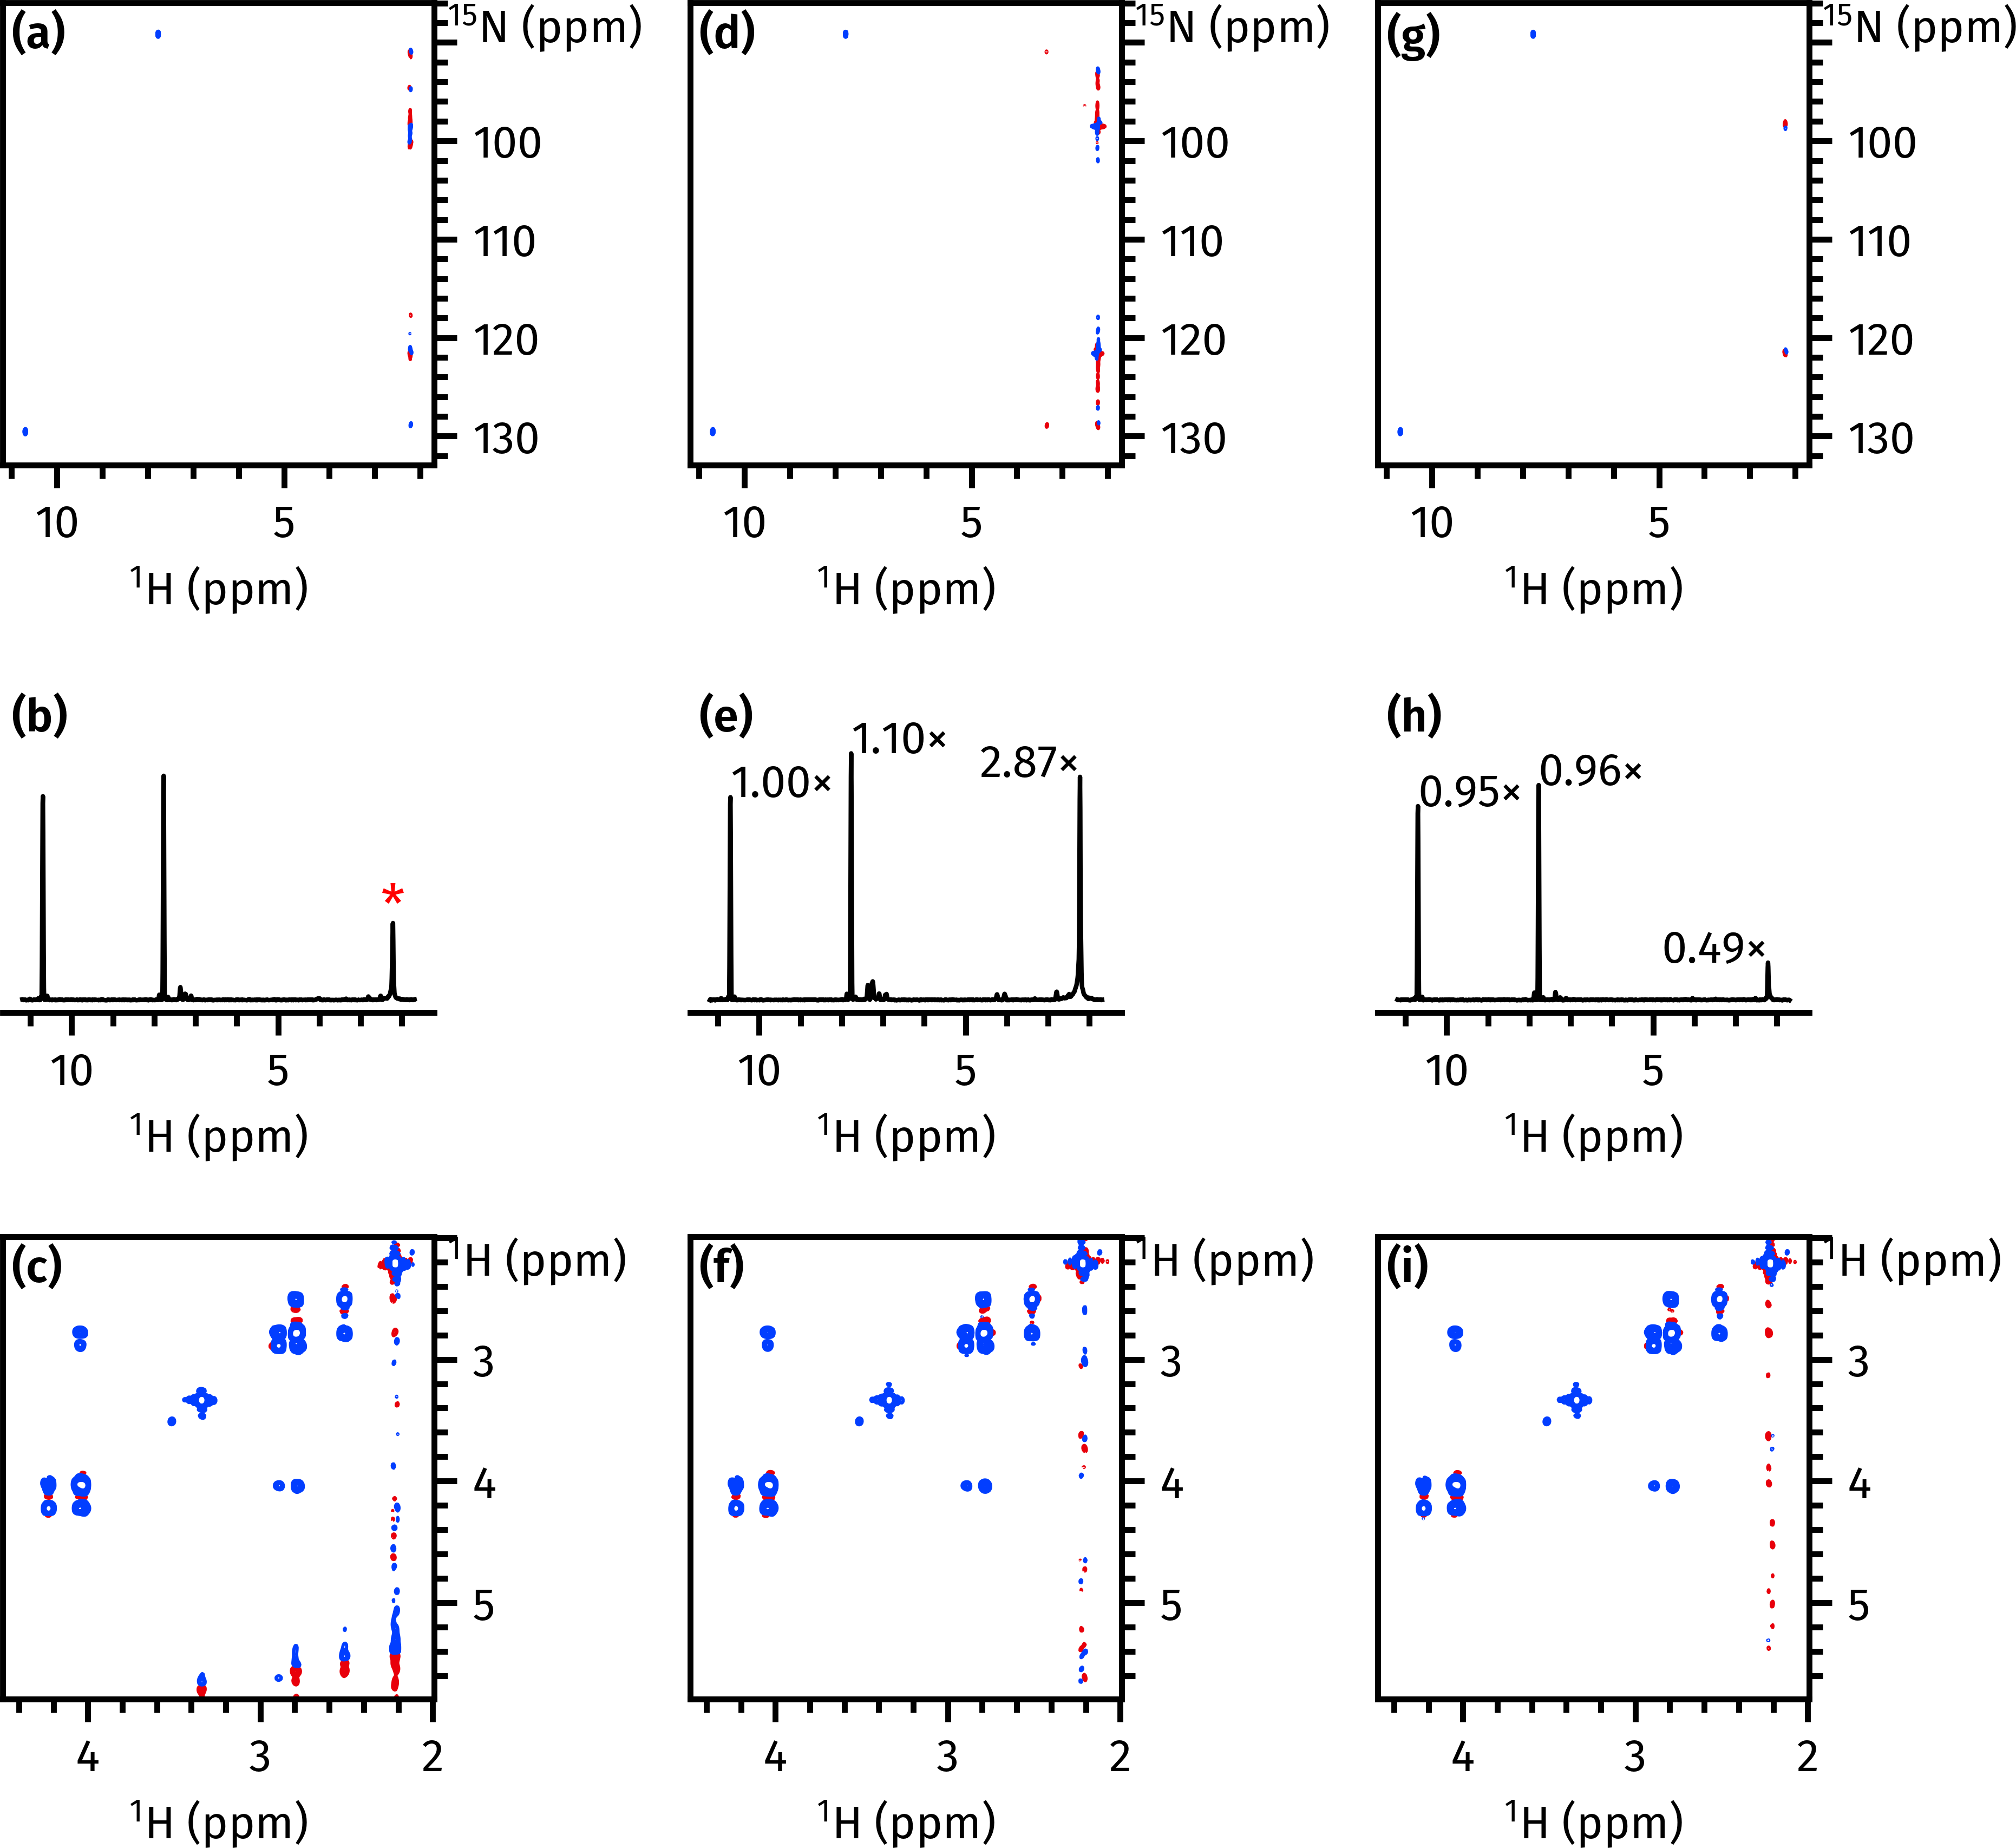
\includegraphics[]{noah/hmqc_grad.png}%
    {\phantomsubcaption\label{fig:hmqc_grad_spec_4grad_1ms_hmqc}}%
    {\phantomsubcaption\label{fig:hmqc_grad_spec_4grad_1ms_hmqcp}}%
    {\phantomsubcaption\label{fig:hmqc_grad_spec_4grad_1ms_cosy}}%
    {\phantomsubcaption\label{fig:hmqc_grad_spec_2grad_1ms_hmqc}}%
    {\phantomsubcaption\label{fig:hmqc_grad_spec_2grad_1ms_hmqcp}}%
    {\phantomsubcaption\label{fig:hmqc_grad_spec_2grad_1ms_cosy}}%
    {\phantomsubcaption\label{fig:hmqc_grad_spec_2grad_2p5ms_hmqc}}%
    {\phantomsubcaption\label{fig:hmqc_grad_spec_2grad_2p5ms_hmqcp}}%
    {\phantomsubcaption\label{fig:hmqc_grad_spec_2grad_2p5ms_cosy}}%
    \caption[Comparison of \noah{Mn,Sp,Cc} modules with different HMQC gradient schemes]{
        Comparison of HMQC and CLIP-COSY spectra obtained from \noah{Mn,Sp,Cc} supersequences, acquired using different HMQC gradient schemes.
        In the first row, the HMQC spectrum itself is shown.
        In the second row, the positive projection of the HMQC spectrum onto the $F_2$ axis is shown; the numbers indicate peak intensities with respect to the reference dataset (the left column).
        The asterisks indicate artefacts arising from bulk magnetisation which is not sufficiently dephased by the final gradient.
        In the third row, (an inset of) the CLIP-COSY spectrum is shown.
        \textbf{(\subref*{fig:hmqc_grad_spec_4grad_1ms_hmqc})--(\subref*{fig:hmqc_grad_spec_4grad_1ms_cosy})} Using the four-gradient scheme of \cref{fig:noah_hmqc_4grad}, with \qty{1}{ms} gradients.
        \textbf{(\subref*{fig:hmqc_grad_spec_2grad_1ms_hmqc})--(\subref*{fig:hmqc_grad_spec_2grad_1ms_cosy})} Using the two-gradient scheme of \cref{fig:noah_hmqc_2grad}, with \qty{1}{ms} gradients.
        \textbf{(\subref*{fig:hmqc_grad_spec_2grad_2p5ms_hmqc})--(\subref*{fig:hmqc_grad_spec_2grad_2p5ms_cosy})} Using the two-gradient scheme of \cref{fig:noah_hmqc_2grad}, with \qty{2.5}{ms} gradients.
        \datacode{7Z-200926}
    }
    \label{fig:hmqc_grad_spec}
\end{figure}

It is of some interest to check whether such a long gradient is truly required.
I therefore ran the two-gradient HMQC experiment with a series of gradient durations from \qty{1}{\ms} to \qty{2.5}{\ms}; the signal and artefact intensities in each of these experiments are plotted in \cref{fig:hmqc_cnst16}.
Generally, there is little variation in the intensities of the two desired peaks.
The artefact intensity is more erratic, which possibly reflects the fact that gradient dephasing varies sinusoidally with the gradient duration $\tau$ due to the spatial integral
\begin{equation}
    \label{eq:gradient_dephasing}
    \frac{1}{L} \int_{-L/2}^{L/2} \exp(\mi \gamma Gz\tau)\,\mathrm{d}z = \frac{\sin(\gamma G L\tau/2)}{\gamma GL\tau/2},
\end{equation}
where $L$ is the sample length and $G$ the gradient amplitude (see also \cref{eq:density_operator_integration}).
Nevertheless, there is a clear decrease in the signal intensity as the gradient duration increases, which (at least in these datasets) is greatest with \qty{2.5}{\ms} gradients.
Since the signal intensity is not affected much, I deemed this to be a perfectly suitable value.

\begin{figure}[!ht]
    \centering
    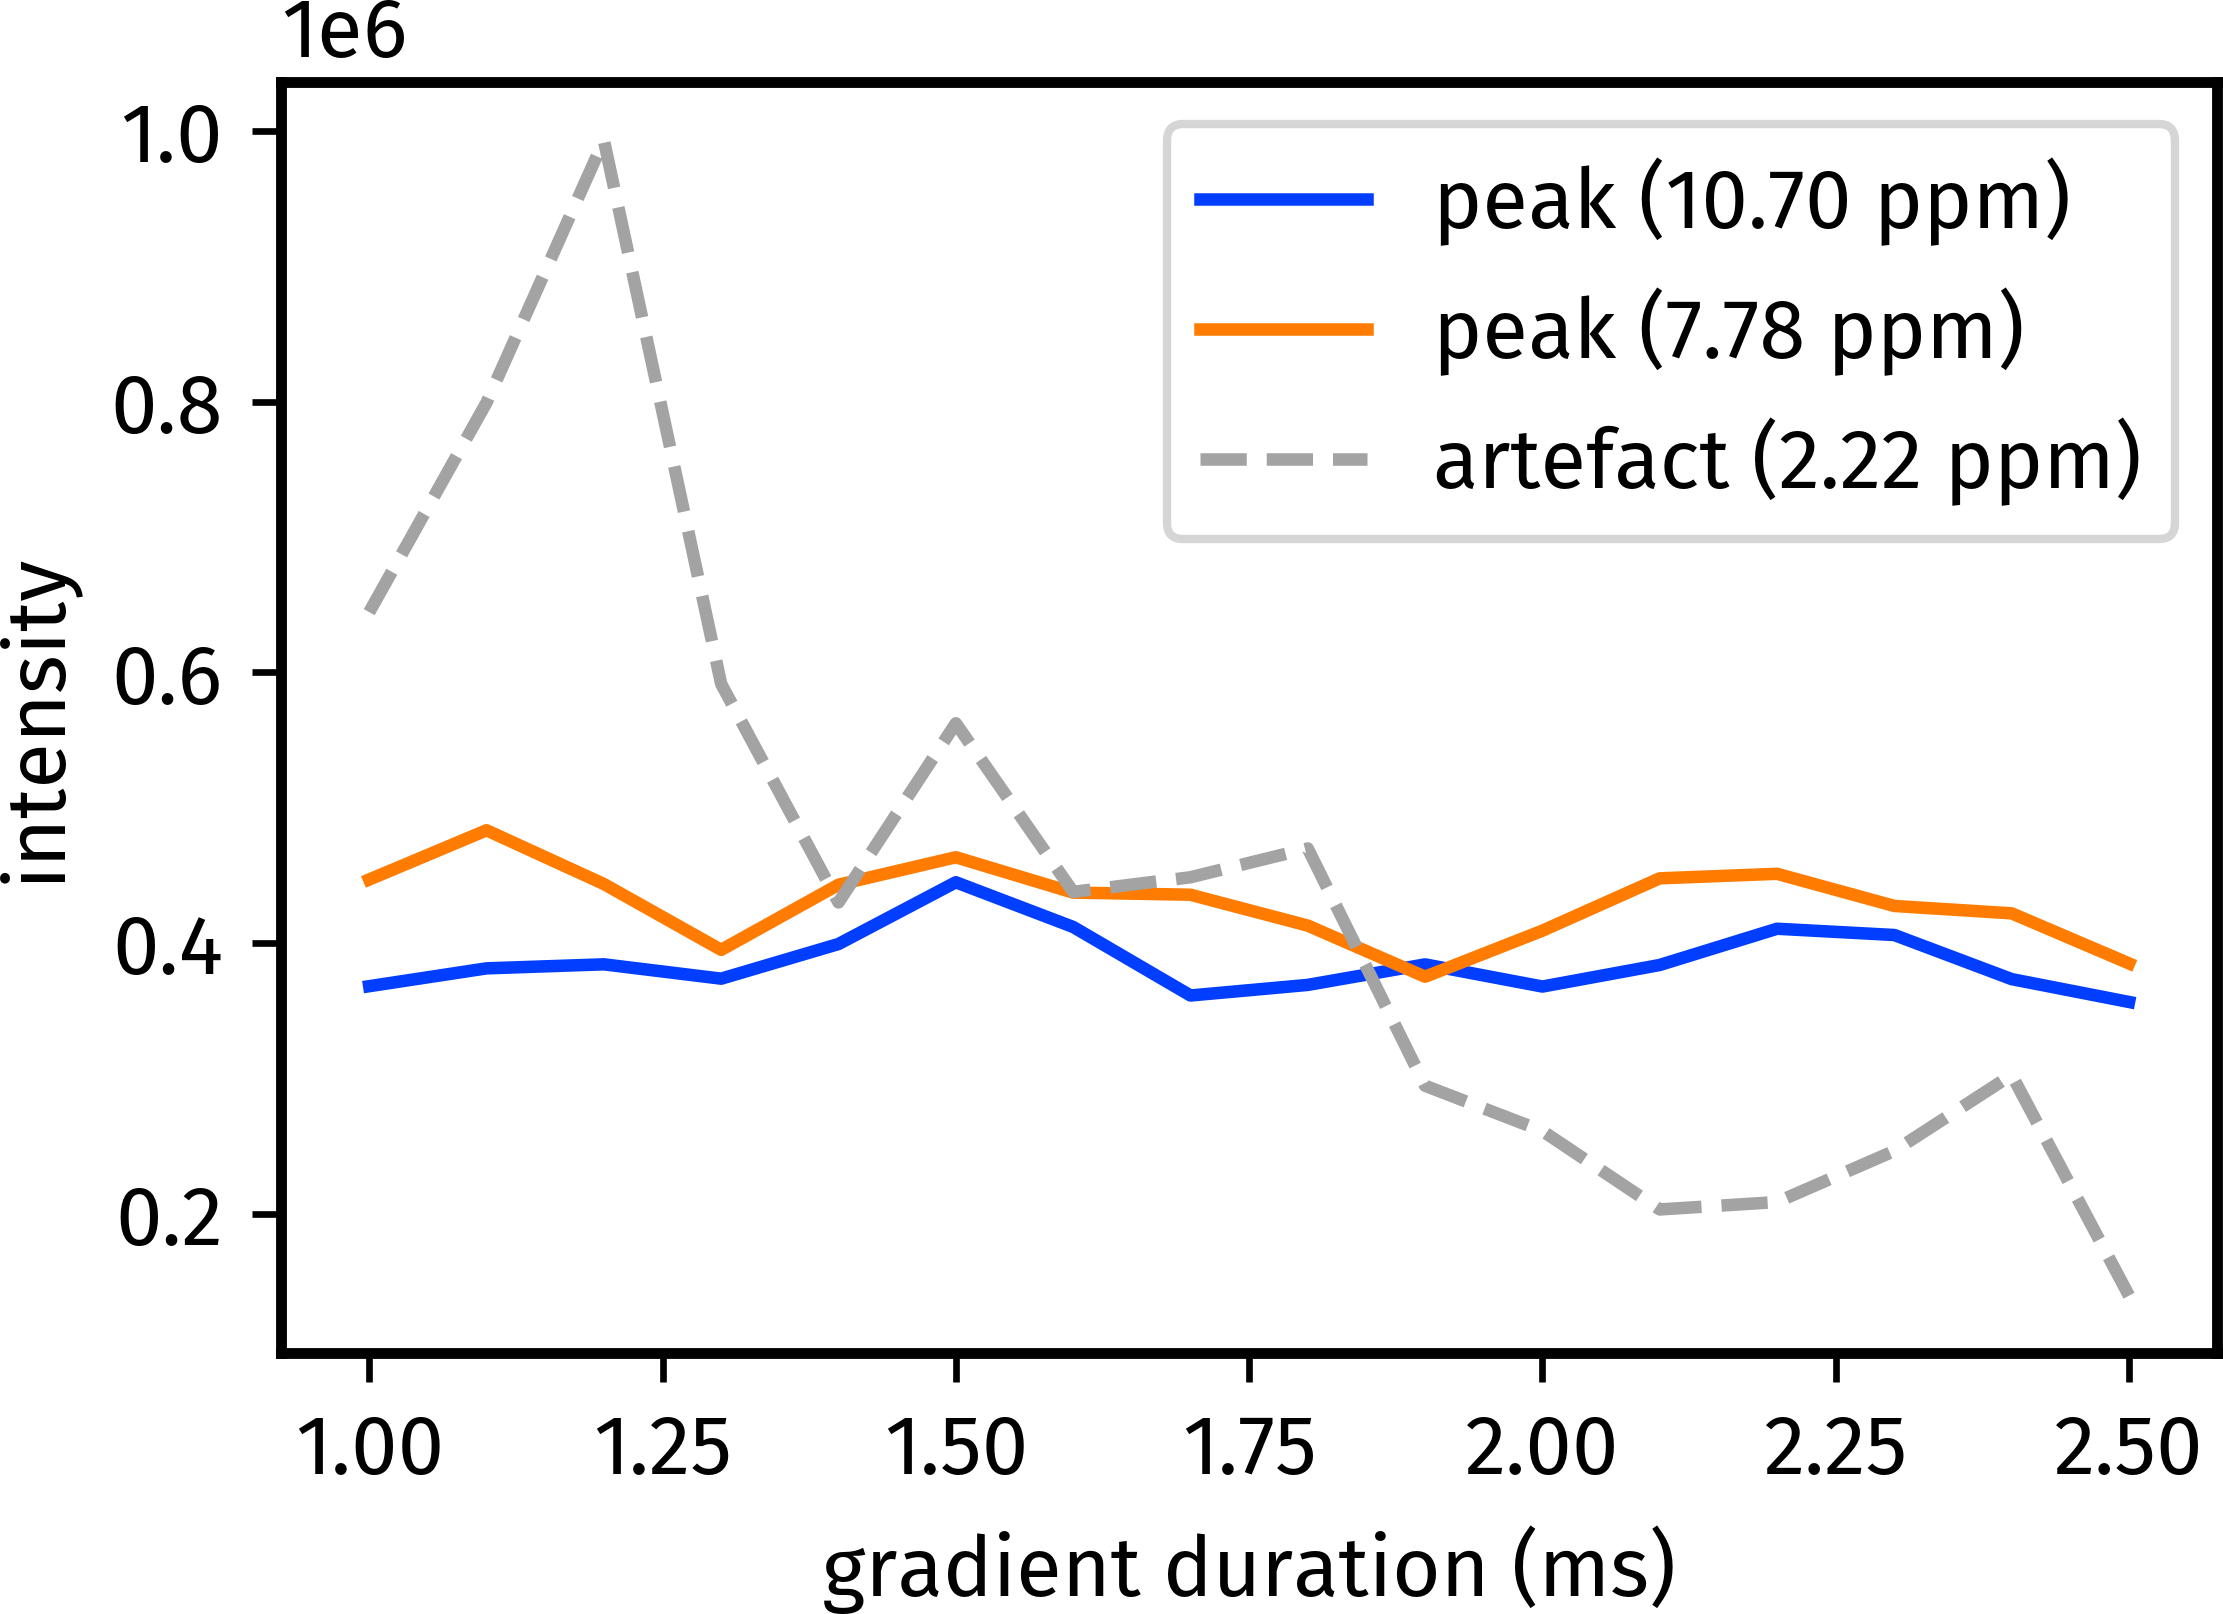
\includegraphics[]{noah/hmqc_cnst16_scan.png}%
    \caption[Variation of HMQC signal and artefact intensity with CTP gradient duration]{
        Variation of HMQC signal and artefact intensity with CTP gradient duration, as measured by (absolute) peak heights in the positive $F_2$ projection.
        \datacode{7Z-200926}
    }
    \label{fig:hmqc_cnst16}
\end{figure}



\subsubsection{$\symbfit{k}$- and SW-scaling}

\proton{}--\nitrogen{} spectra of small molecules are often relatively sparse in the indirect dimension, and do not typically need to be acquired with the same resolution as a \proton{}--\carbon{} experiment.
However, if these experiments were to be combined together within a supersequence, it is not ordinarily possible to toggle the resolution of each module individually.
One way of circumventing this issue is to decrease the frequency with which the \nitrogen{} $t_1$ duration is incremented in the pulse programme: this was first proposed by Parella et al.\ in the context of time-shared NMR\autocite{PerezTrujillo2007MRC,Parella2010CMR}, and in this thesis is called `$k$-scaling'.
This means that each $t_1$ increment is acquired several times before $t_1$ is incremented; effectively leading to $k$ times fewer $t_1$ increments, but with each increment having $k$ times the number of scans (after the data have been combined).
An alternative is to simply increase the spectral width of the \nitrogen{} module (which is encoded as the \texttt{CNST40} parameter in GENESIS).

\begin{figure}[!ht]
    \centering
    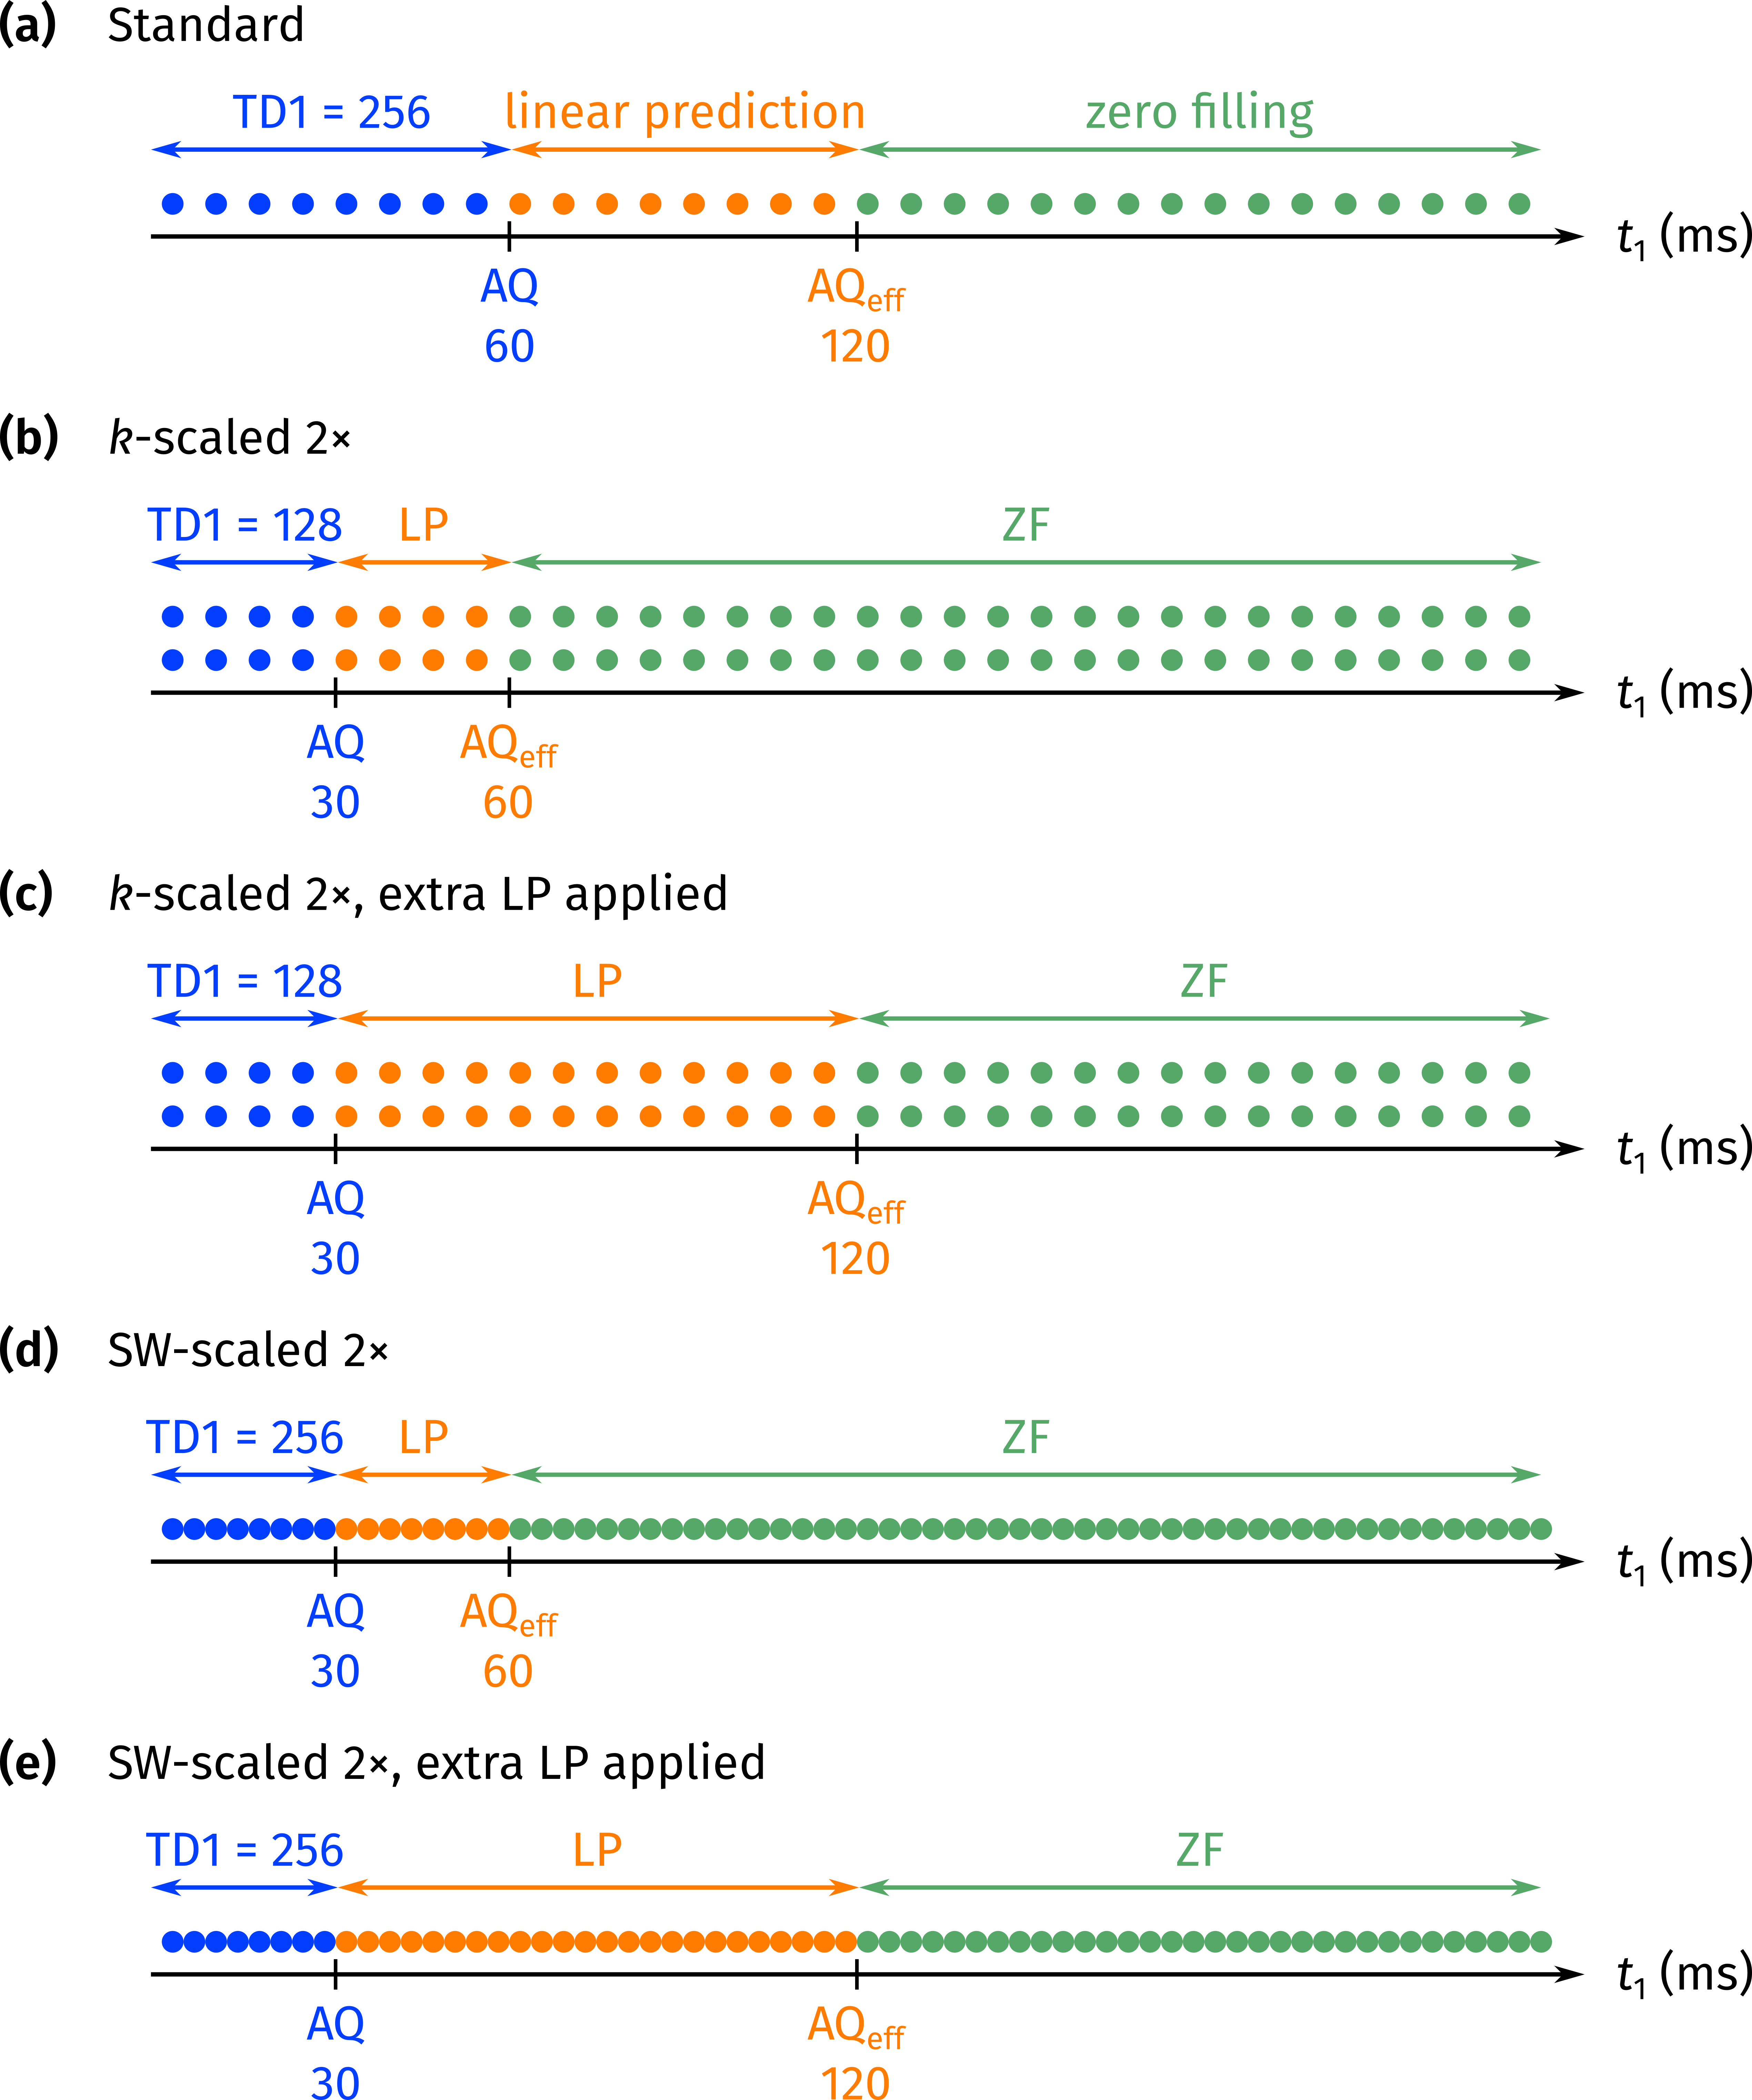
\includegraphics[]{noah/n15_t1_diagram.png}%
    {\phantomsubcaption\label{fig:n15_t1_normal}}%
    {\phantomsubcaption\label{fig:n15_t1_k}}%
    {\phantomsubcaption\label{fig:n15_t1_k_lp}}%
    {\phantomsubcaption\label{fig:n15_t1_sw}}%
    {\phantomsubcaption\label{fig:n15_t1_sw_lp}}%
    \caption[Pictorial representation of $k$- and SW-scaling in NOAH \nitrogen{} modules]{
        Pictorial representation of $k$- and SW-scaling in NOAH \nitrogen{} modules.
        Each blue dot represents 32 $t_1$ increments physically acquired as part of the experiment; the experimental time is proportional to the number of blue dots, and is constant across all of these experiments.
        Orange dots represent 32 $t_1$ increments obtained through forward linear prediction, and green dots represent zeroes.
        \textbf{(\subref*{fig:n15_t1_normal})} The default experiment.
        \textbf{(\subref*{fig:n15_t1_k})--(\subref*{fig:n15_t1_k_lp})} $k$-scaled experiment, without and with extra linear processing to restore the original value of $\AQeff$.
        \textbf{(\subref*{fig:n15_t1_sw})--(\subref*{fig:n15_t1_sw_lp})} SW-scaled experiment, without and with extra linear processing to restore the original value of $\AQeff$.
    }
    \label{fig:n15_t1}
\end{figure}

\Cref{fig:n15_t1} illustrates all of these possibilities in detail.
In a `typical' NOAH supersequence (\cref{fig:n15_t1_normal}), 256 $t_1$ increments would be recorded (corresponding to the eight blue dots);
for the gramicidin sample used here, the largest value of $t_1$ (denoted as $\AQ$) is around \qty{60}{\ms}.
The default TopSpin processing routine for 2D NMR applies forward linear prediction (LP)\autocite{Ni1986JMR,Tirendi1989JMR,Led1991CR,Koehl1999PNMRS} in the indirect dimension, such as to double the number of points: the data points obtained through LP are indicated by orange dots.
This leads to an \textit{effective} $\AQ$ which is twice as large, denoted as $\AQeff$.
Finally, zero filling (ZF) is applied to increase the digital resolution to a given value, as represented by the green dots.

In the $k$-scaled spectrum, both $\AQ$ (and thus $\AQeff$) are halved, in return for a doubling of the number of scans (\cref{fig:n15_t1_k}).
The resolution in the indirect dimension is proportional to $\AQeff$; thus, this also corresponds to a $2\times$ decrease in resolution.
However, this can be counteracted through the use of extra linear prediction (\cref{fig:n15_t1_k_lp}) to extend $\AQeff$ back to its original value.
The SW-scaled spectra (\cref{fig:n15_t1_sw,fig:n15_t1_sw_lp}) are almost entirely equivalent to the $k$-scaled spectra in terms of their effect on $\AQ$ and $\AQeff$, except that the sampling schedule is very slightly modified.

\Cref{fig:hmqc_scale} shows the effects of performing $k$- or SW-scaling on the \nitrogen{} HMQC module (without any extra linear prediction beyond the default).
In this case, these scaling procedures can in fact can lead to significant gains in SNR (as measured by peak heights), with up to $2.6\times$ improvements being observed at the extreme of 8-fold $k$- or SW-scaling.
This likely arises because the $J_{\ch{HH}}$ modulation in the indirect dimension (visible in the standard spectrum, \cref{fig:hmqc_scale_std1}) is no longer being resolved: the largest gains are attained for the peak at \qty{123}{\ppm}, where this modulation is especially prominent.

\begin{figure}[!htbp]
    \centering
    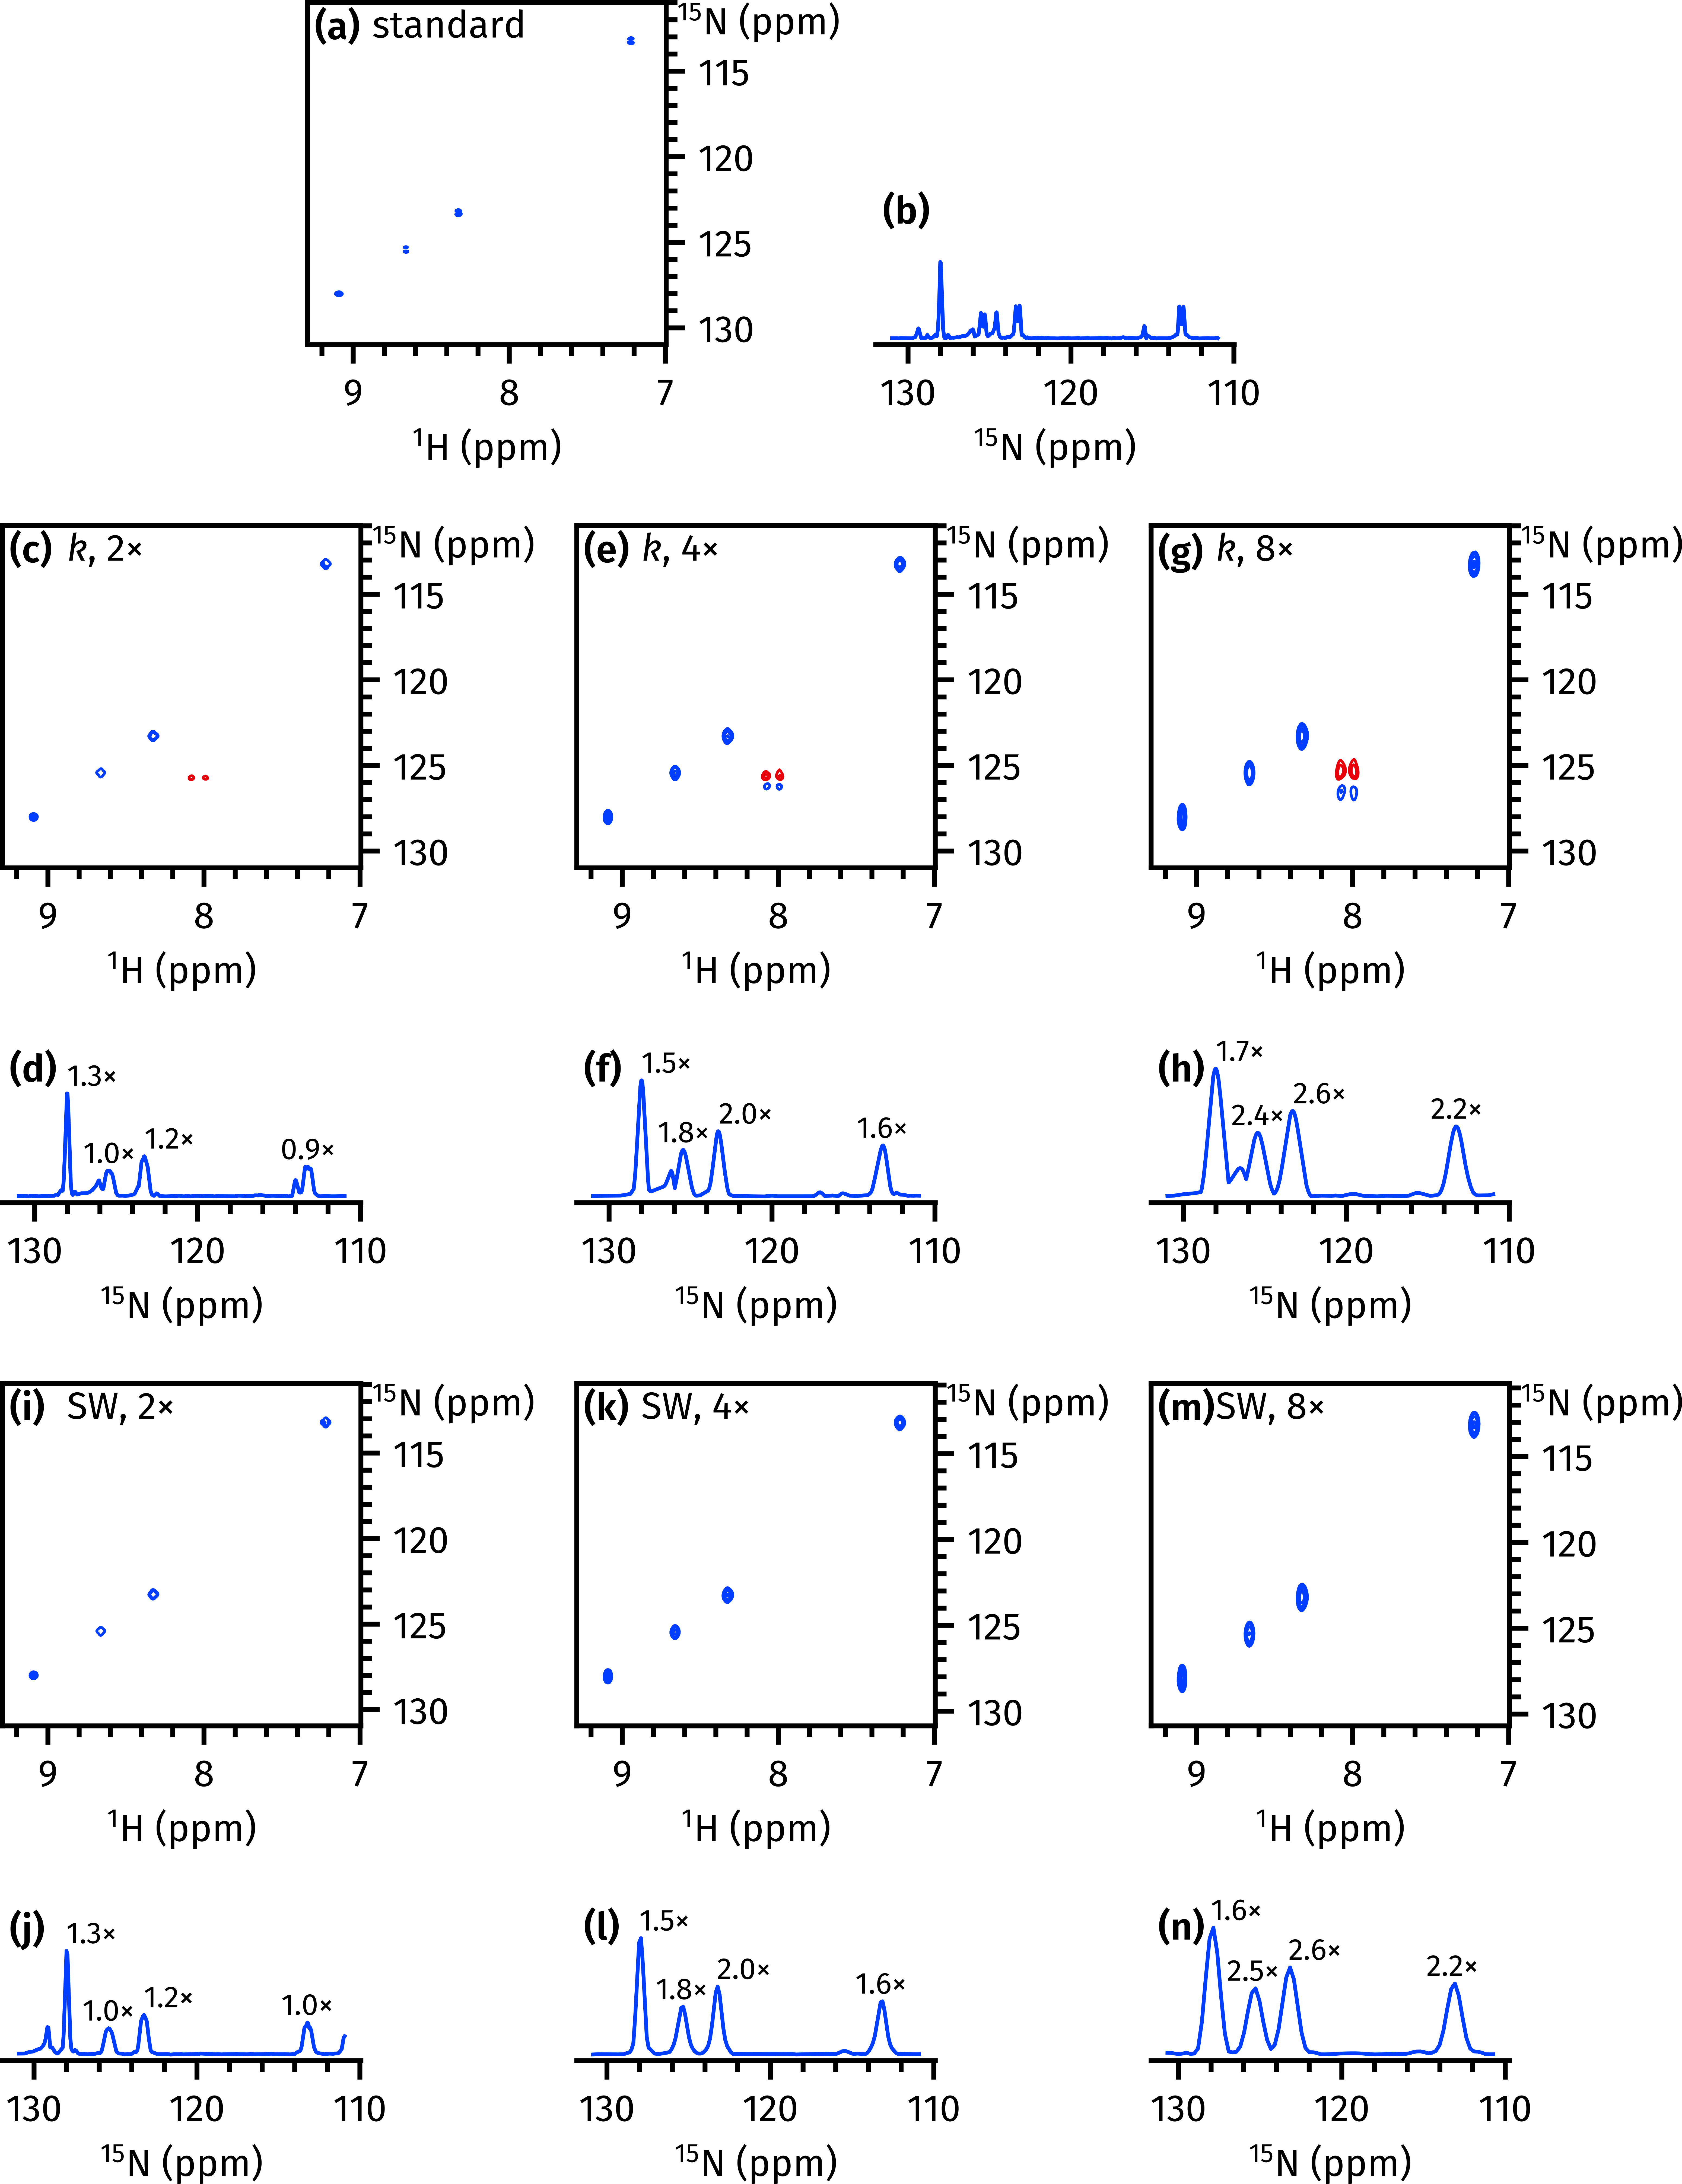
\includegraphics[]{noah/hmqc_scale.png}%
    {\phantomsubcaption\label{fig:hmqc_scale_std2}}%
    {\phantomsubcaption\label{fig:hmqc_scale_std1}}%
    {\phantomsubcaption\label{fig:hmqc_scale_k22}}%
    {\phantomsubcaption\label{fig:hmqc_scale_k21}}%
    {\phantomsubcaption\label{fig:hmqc_scale_k42}}%
    {\phantomsubcaption\label{fig:hmqc_scale_k41}}%
    {\phantomsubcaption\label{fig:hmqc_scale_k82}}%
    {\phantomsubcaption\label{fig:hmqc_scale_k81}}%
    {\phantomsubcaption\label{fig:hmqc_scale_sw22}}%
    {\phantomsubcaption\label{fig:hmqc_scale_sw21}}%
    {\phantomsubcaption\label{fig:hmqc_scale_sw42}}%
    {\phantomsubcaption\label{fig:hmqc_scale_sw41}}%
    {\phantomsubcaption\label{fig:hmqc_scale_sw82}}%
    {\phantomsubcaption\label{fig:hmqc_scale_sw81}}%
    \caption[Effects of $k$- and SW-scaling on NOAH HMQC spectrum]{
        Effects of $k$- and SW-scaling on NOAH HMQC spectrum (taken from \noah{Mn,Sp,Cc} supersequences).
        Each HMQC spectrum is shown together with a positive projection onto the $F_1$ axis.
        The relative SNR of each peak, with respect to the standard spectrum, is indicated on each of the other projections.
        \textbf{(\subref*{fig:hmqc_scale_std2})--(\subref*{fig:hmqc_scale_std1})} Standard spectrum.
        \textbf{(\subref*{fig:hmqc_scale_k22})--(\subref*{fig:hmqc_scale_k81})} $k$-scaled spectra.
        \textbf{(\subref*{fig:hmqc_scale_sw22})--(\subref*{fig:hmqc_scale_sw81})} SW-scaled spectra.
        \datacode{7G-210310}
    }
    \label{fig:hmqc_scale}
\end{figure}

The effect of adding extra linear prediction is shown in \cref{fig:hmqc_scale_lp}.
In general, the combination of scaling plus LP leads to improvements in spectral SNR of up to $6\times$.
However, this is accompanied by distortions in the $F_1$ multiplet structure, especially for the $k$-scaled spectra (\cref{fig:hmqc_scale_lp_k22,fig:hmqc_scale_lp_k21,fig:hmqc_scale_lp_k42,fig:hmqc_scale_lp_k41,fig:hmqc_scale_lp_k82,fig:hmqc_scale_lp_k81}): it is possible that the corresponding SW-scaled spectra are not so heavily distorted because there are more data points to extrapolate from.

However, caution should be exercised when interpreting these results.
Although this improvement in SNR is genuine, it is not necessarily the case that this represents a true improvement in \textit{detection sensitivity}: in other words, processing techniques such as LP (and to some extent, NUS) do not always allow for better discrimination between signal and noise.\autocite{Donoho1990PNASUSA,Stern2002JACS}%
\footnote{In recent years, this issue has been investigated more thoroughly in the context of NUS.\autocite{Palmer2015JPCB}}
Further tests would need to be done on more dilute samples\footnote{Or, perhaps, less sensitive instruments---although the \qty{700}{\MHz} cryoprobe used here was the only option for these supersequences.} to ascertain the benefits of the scaling-plus-LP routine on spectra with less intrinsic SNR.

\begin{figure}[!htbp]
    \centering
    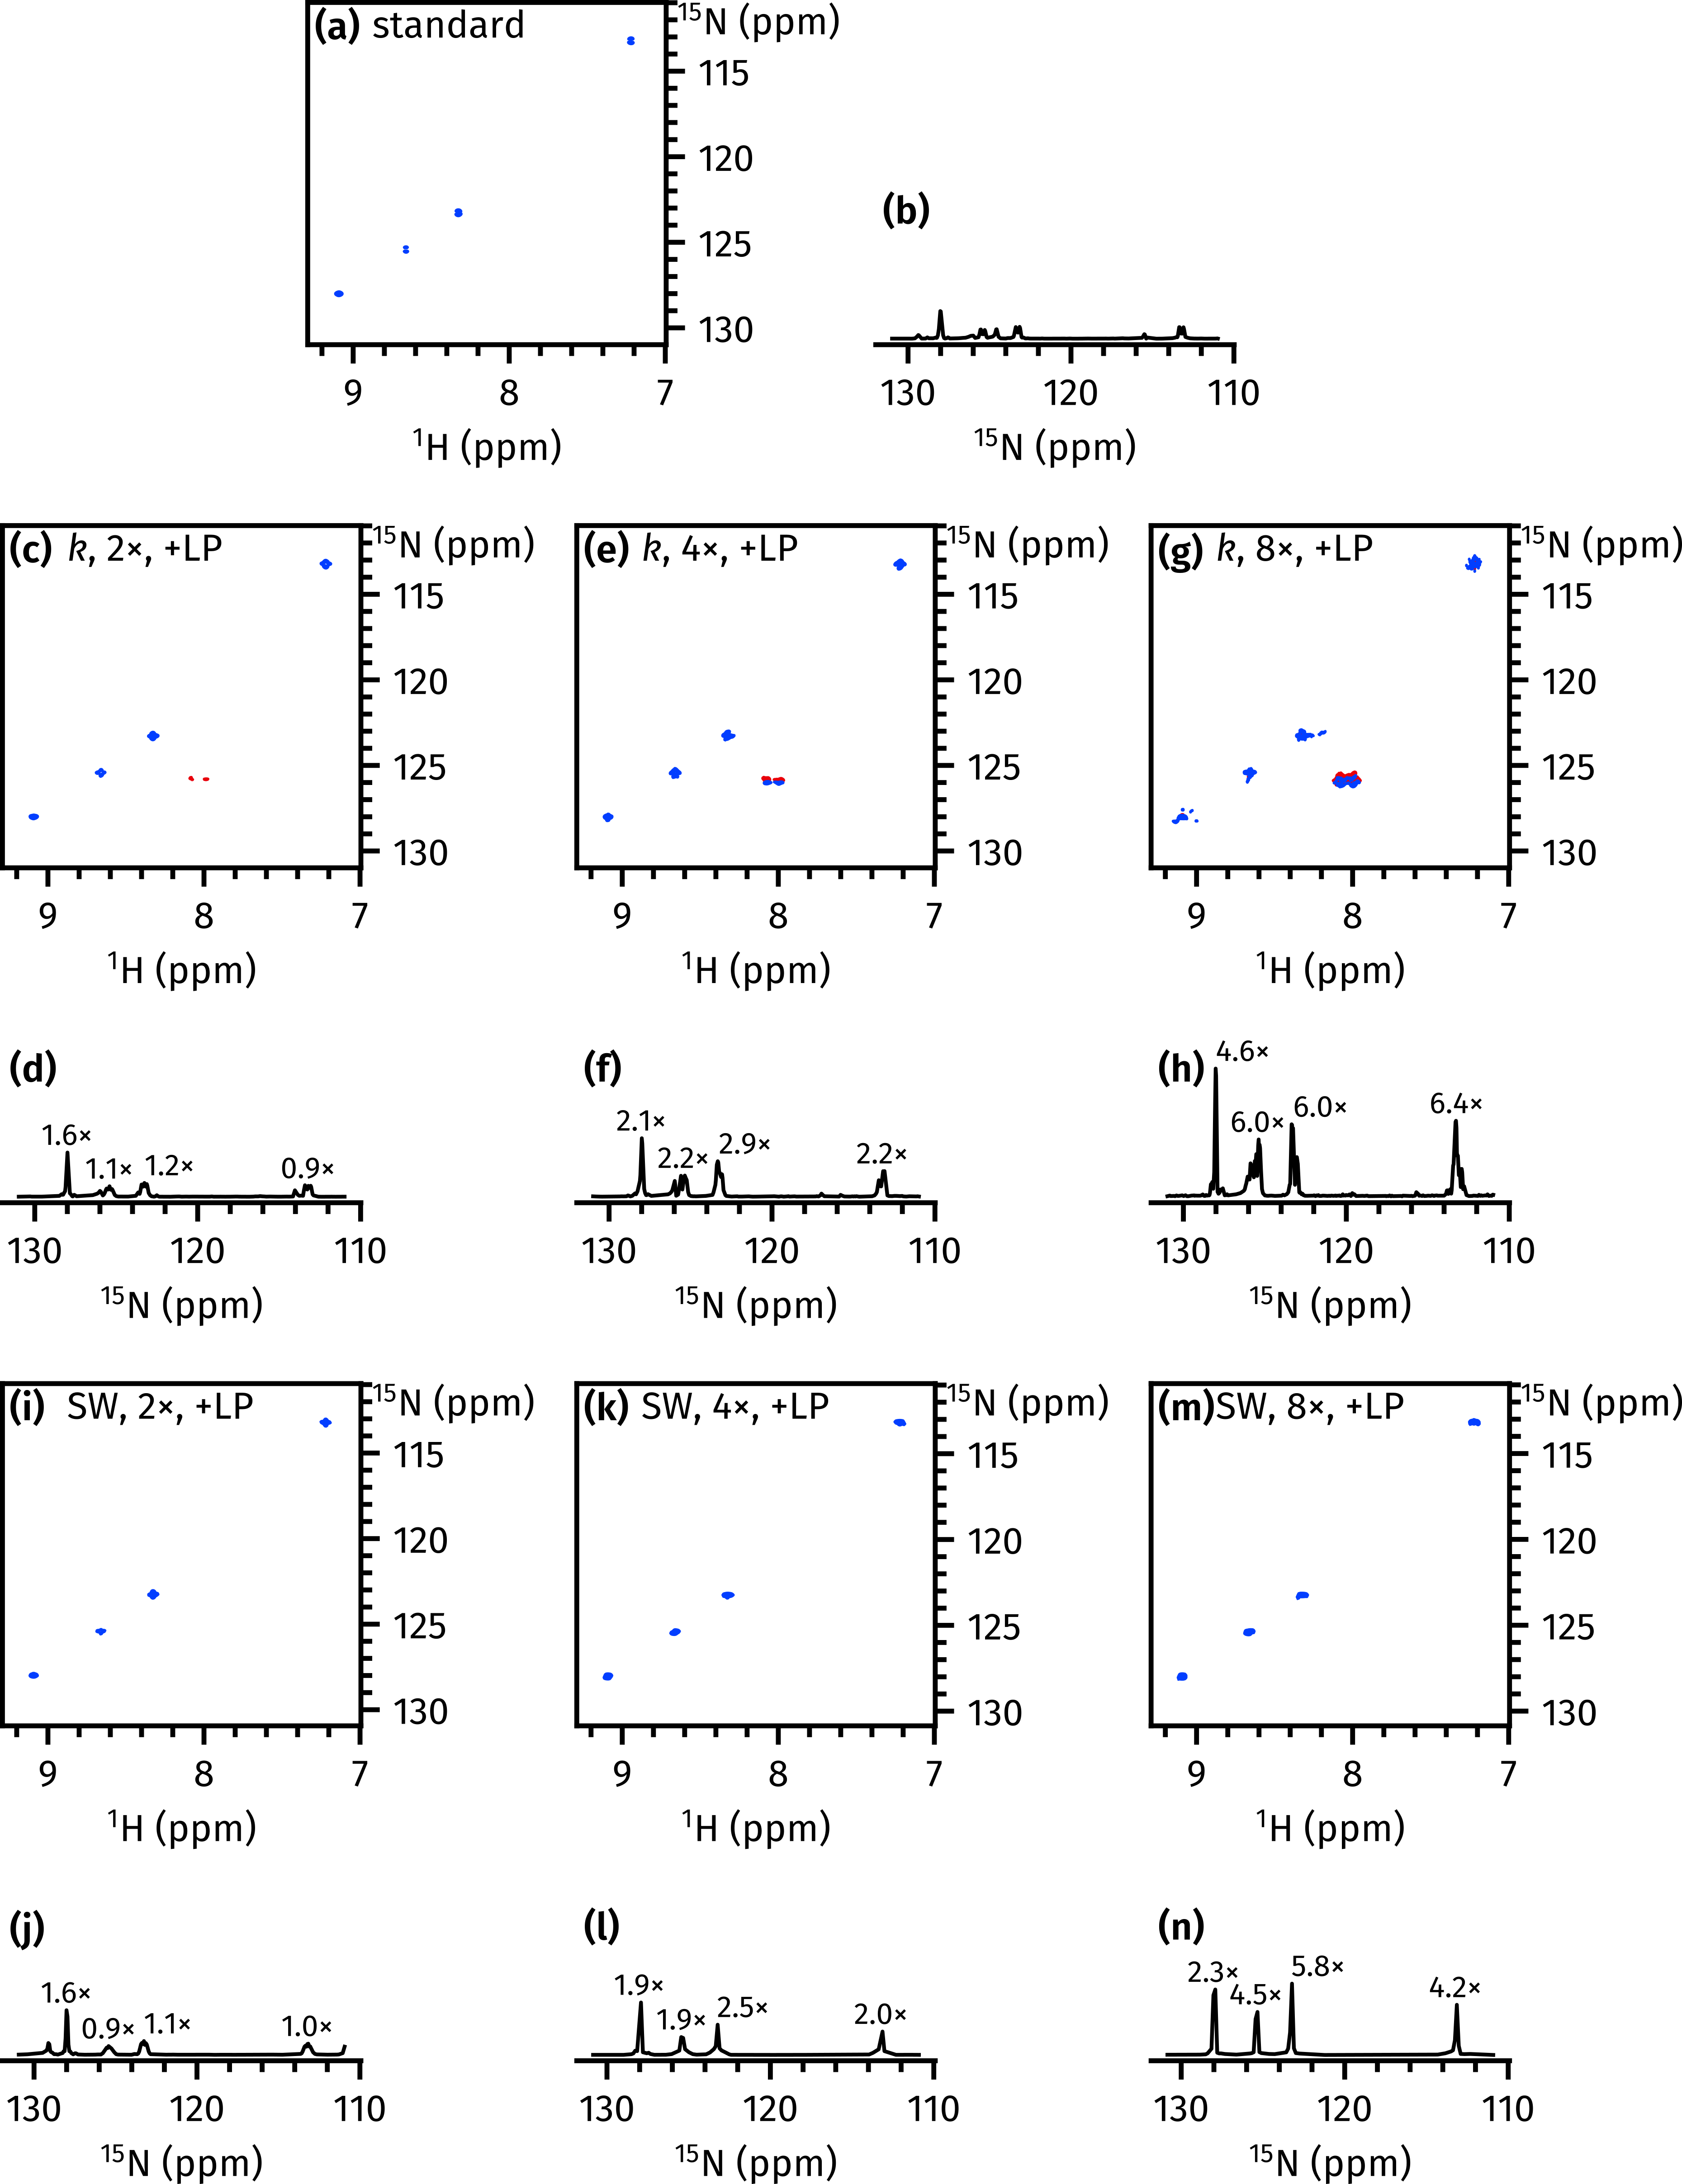
\includegraphics[]{noah/hmqc_scale_lp.png}%
    {\phantomsubcaption\label{fig:hmqc_scale_lp_std2}}%
    {\phantomsubcaption\label{fig:hmqc_scale_lp_std1}}%
    {\phantomsubcaption\label{fig:hmqc_scale_lp_k22}}%
    {\phantomsubcaption\label{fig:hmqc_scale_lp_k21}}%
    {\phantomsubcaption\label{fig:hmqc_scale_lp_k42}}%
    {\phantomsubcaption\label{fig:hmqc_scale_lp_k41}}%
    {\phantomsubcaption\label{fig:hmqc_scale_lp_k82}}%
    {\phantomsubcaption\label{fig:hmqc_scale_lp_k81}}%
    {\phantomsubcaption\label{fig:hmqc_scale_lp_sw22}}%
    {\phantomsubcaption\label{fig:hmqc_scale_lp_sw21}}%
    {\phantomsubcaption\label{fig:hmqc_scale_lp_sw42}}%
    {\phantomsubcaption\label{fig:hmqc_scale_lp_sw41}}%
    {\phantomsubcaption\label{fig:hmqc_scale_lp_sw82}}%
    {\phantomsubcaption\label{fig:hmqc_scale_lp_sw81}}%
    \caption[Effects of $k$- and SW-scaling on NOAH HMQC spectrum with extra linear prediction]{
        The same as in \cref{fig:hmqc_scale}, but with extra linear prediction applied to all scaled spectra to bring $\AQeff$ up to its original value in the standard spectrum.
        Linear prediction of $k$ times more points leads to a $\sqrt{k}$ increase in noise; to account for this, all spectra are plotted with the same noise level.
        \textbf{(\subref*{fig:hmqc_scale_lp_std2})--(\subref*{fig:hmqc_scale_lp_std1})} Standard spectrum.
        \textbf{(\subref*{fig:hmqc_scale_lp_k22})--(\subref*{fig:hmqc_scale_lp_k81})} $k$-scaled spectra.
        \textbf{(\subref*{fig:hmqc_scale_lp_sw22})--(\subref*{fig:hmqc_scale_lp_sw81})} SW-scaled spectra.
        \datacode{7G-210310}
    }
    \label{fig:hmqc_scale_lp}
\end{figure}
